% !TeX program = xelatex
\documentclass[a4paper,10pt]{article}

% ============================================================================
% ១. កញ្ចប់បណ្ណាល័យ និងការកំណត់ទំព័រ (Packages & Page Setup — តាមគំរូ ls_plan.tex)
% ============================================================================
\usepackage[a4paper, left=0.95cm, right=0.95cm, top=0.85cm, bottom=0.92cm, footskip=0.52cm]{geometry}
\usepackage{amsmath}
\usepackage{unicode-math}
\usepackage{fontspec}
\usepackage{longtable, array, multirow, colortbl}
\usepackage[table]{xcolor}
\usepackage{enumitem}
\usepackage{pifont}
\usepackage{fancyhdr}
\usepackage{tikz}
\usetikzlibrary{calc, arrows.meta, decorations.pathreplacing, patterns, positioning, babel}

\makeatletter
\let\@expl@@@mark@update@singlecol@structures@@\relax
\makeatother

% --- ប្រព័ន្ធស្វែងរកទីតាំងពុម្ពអក្សរស្វ័យប្រវត្តិ (Windows Local + Cloud Repo fonts/) ---
\providecommand{\NGSFindFonts}{%
  \IfFileExists{C:/Windows/Fonts/cambria.ttc}{%
    \def\NGSSysPath{C:/Windows/Fonts/}%
    \def\NGSUserPath{C:/Users/KIT/AppData/Local/Microsoft/Windows/Fonts/}%
  }{%
    \IfFileExists{./fonts/KhmerOSsiemreap.ttf}{\def\NGSSysPath{./fonts/}\def\NGSUserPath{./fonts/}}{%
    \IfFileExists{../fonts/KhmerOSsiemreap.ttf}{\def\NGSSysPath{../fonts/}\def\NGSUserPath{../fonts/}}{%
    \IfFileExists{../../fonts/KhmerOSsiemreap.ttf}{\def\NGSSysPath{../../fonts/}\def\NGSUserPath{../../fonts/}}{%
    \IfFileExists{../../../fonts/KhmerOSsiemreap.ttf}{\def\NGSSysPath{../../../fonts/}\def\NGSUserPath{../../../fonts/}}{%
    \IfFileExists{../../../../fonts/KhmerOSsiemreap.ttf}{\def\NGSSysPath{../../../../fonts/}\def\NGSUserPath{../../../../fonts/}}{%
    \IfFileExists{../../../../../fonts/KhmerOSsiemreap.ttf}{\def\NGSSysPath{../../../../../fonts/}\def\NGSUserPath{../../../../../fonts/}}{%
    \IfFileExists{../../../../../../fonts/KhmerOSsiemreap.ttf}{\def\NGSSysPath{../../../../../../fonts/}\def\NGSUserPath{../../../../../../fonts/}}{%
      \def\NGSSysPath{../../../../../../../fonts/}\def\NGSUserPath{../../../../../../../fonts/}%
    }}}}}}}%
  }%
}
\NGSFindFonts

% ============================================================================
% ២. កំណត់ពុម្ពអក្សរ (Fonts — តាមគំរូ ls_plan.tex)
% ============================================================================
\setmathfont[Path={\NGSSysPath}, FontIndex=1, Scale=1.02]{cambria.ttc}
\defaultfontfeatures{Ligatures=TeX}

\setmainfont[
  Path={\NGSUserPath},
  Extension=.ttf,
  Script=Khmer,
  BoldFont={KhmerOSsiemreap},
  BoldFeatures={FakeBold=1.8},
  ItalicFont={KhmerOSsiemreap},
  ItalicFeatures={FakeSlant=0.25},
  BoldItalicFont={KhmerOSsiemreap},
  BoldItalicFeatures={FakeBold=1.8, FakeSlant=0.25}
]{KhmerOSsiemreap}

\newfontfamily\muol[Path={\NGSUserPath}, Extension=.ttf, Script=Khmer]{KhmerOSmuollight}
\newfontfamily\Tacteing[Path={\NGSUserPath}, Extension=.TTF]{TACTENG}
\newfontfamily\TimesEn[Path={\NGSSysPath}, Extension=.ttf, BoldFont={timesbd}, ItalicFont={timesi}, BoldItalicFont={timesbi}]{times}
\newfontfamily\CalibriFont[Path={\NGSSysPath}, Extension=.ttf]{calibri}
\newfontfamily\CourierCirc[Path={\NGSSysPath}, Extension=.ttf]{cour}

\XeTeXlinebreaklocale "km"
\XeTeXlinebreakskip = 0pt plus 1pt minus 0.1pt

% ============================================================================
% ៣. ពណ៌ និងការតុបតែង (Colors & Styles)
% ============================================================================
\definecolor{stepbg}{HTML}{D9D9D9}
\definecolor{headgray}{HTML}{E6E6E6}
\definecolor{emphred}{HTML}{C00000}

\pagestyle{fancy}
\fancyhf{}
\renewcommand{\headrulewidth}{0pt}
\fancyfoot[R]{\CalibriFont\fontsize{9pt}{11pt}\selectfont\thepage}

\setlength{\parindent}{0pt}
\setlength{\parskip}{0pt}
\setlength{\tabcolsep}{4.5pt}
\setlength{\LTpre}{2pt}
\setlength{\LTpost}{2pt}

\newcolumntype{L}[1]{>{\raggedright\arraybackslash}p{#1}}
\newcolumntype{C}[1]{>{\centering\arraybackslash}p{#1}}

% ============================================================================
% ៤. ពាក្យបញ្ជាជំនួយ (Helper Macros)
% ============================================================================
\newcommand{\en}[1]{{\TimesEn #1}}
\newcommand{\enbf}[1]{{\TimesEn\bfseries #1}}
\newcommand{\khmflourish}{{\Tacteing\fontsize{15pt}{15pt}\selectfont 3}}
\newcommand{\wcirc}{{\CourierCirc\fontsize{9.5pt}{11pt}\selectfont o}}
\newcommand{\ditem}{{\fontsize{7.5pt}{10pt}\selectfont\ding{117}}\ }
\newcommand{\fiveE}[1]{\textcolor{emphred}{\CalibriFont\bfseries #1}}
\newcommand{\redsub}[1]{\textcolor{emphred}{#1}}
\newcommand{\timenote}[1]{\textcolor{emphred}{\textit{#1}}}
\newcommand{\stepheader}[1]{\multicolumn{3}{|c|}{\cellcolor{stepbg}\muol #1} \\ \hline}
\newcommand{\cfig}[1]{{\centering\vspace{3pt}#1\vspace{3pt}\par}}
\newcommand{\cnum}[1]{\mbox{\fontsize{10.5pt}{12pt}\selectfont\ding{\numexpr181+#1\relax}}}
\newcommand{\unit}[1]{\,\text{\en{#1}}}
\newcommand{\riel}{\,\text{៛}}
\newcommand{\graybox}[1]{\colorbox{headgray}{\strut #1}}

% ============================================================================
% ៥. រូបភាព TikZ ស-ខ្មៅ សម្រាប់បង្រៀនលើក្ដារខៀន និងសន្លឹកកិច្ចការ (B&W Diagrams)
% ============================================================================

% ១. E1 Engage: អន្ទាក់សញ្ញាដកមុខវង់ក្រចកពេលដកពហុធា E - F
\newcommand{\figEngageALGFiveThree}{%
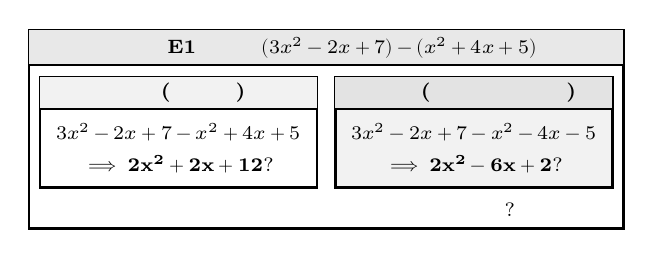
\begin{tikzpicture}[x=1cm, y=1cm, every node/.style={font=\scriptsize, text=black}]
  \draw[black, line width=0.9pt] (0,0) rectangle (7.55,2.52);
  \fill[gray!18] (0,2.08) rectangle (7.55,2.52);
  \draw[black, line width=0.6pt] (0,2.08) -- (7.55,2.08);
  \node at (3.775,2.30) {\textbf{បេសកកម្ម \en{E1}៖ គណនាផលដក $(3x^2 - 2x + 7) - (x^2 + 4x + 5)$}};

  % Student A
  \draw[black, line width=0.8pt] (0.14,0.52) rectangle (3.66,1.92);
  \fill[gray!10] (0.14,1.52) rectangle (3.66,1.92);
  \draw[black, line width=0.5pt] (0.14,1.52) -- (3.66,1.52);
  \node at (1.90,1.72) {\textbf{សិស្ស ក (ប្ដូរតែតួទី១)}};
  \node at (1.90,1.22) {$3x^2 - 2x + 7 - x^2 + 4x + 5$};
  \node at (1.90,0.82) {$\implies \mathbf{2x^2 + 2x + 12}$?};

  % Student B
  \draw[black, line width=0.95pt, fill=gray!10] (3.89,0.52) rectangle (7.41,1.92);
  \fill[gray!22] (3.89,1.52) rectangle (7.41,1.92);
  \draw[black, line width=0.55pt] (3.89,1.52) -- (7.41,1.52);
  \node at (5.65,1.72) {\textbf{សិស្ស ខ (ប្ដូរគ្រប់តួក្នុងវង់ក្រចក)}};
  \node at (5.65,1.22) {$3x^2 - 2x + 7 - x^2 - 4x - 5$};
  \node at (5.65,0.82) {$\implies \mathbf{2x^2 - 6x + 2}$?};

  \node at (3.775,0.24) {\textbf{សំណួរគន្លឹះ៖} ពេលលុបវង់ក្រចកក្រោយសញ្ញាដក តើត្រូវប្ដូរសញ្ញាប៉ុន្មានតួ?};
\end{tikzpicture}}

% ២. E2 Explore: បរិមាត្រត្រីកោណ 3y+2x+8 និងប្រមាណវិធីបូក/ដកជួរឈរ (ទំ.៥៦--៥៩)
\newcommand{\figPolyExploreALGFiveThree}{%
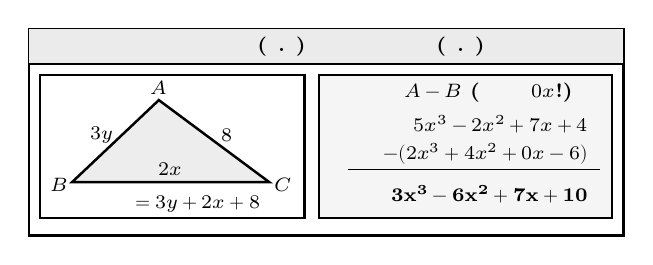
\begin{tikzpicture}[x=1cm, y=1cm, every node/.style={font=\scriptsize, text=black}]
  \draw[black, line width=0.9pt] (0,0) rectangle (7.55,2.62);
  \fill[gray!16] (0,2.18) rectangle (7.55,2.62);
  \draw[black, line width=0.6pt] (0,2.18) -- (7.55,2.18);
  \node at (3.775,2.40) {\textbf{បរិមាត្រត្រីកោណ (ទំ.៥៦) និងការបូកដកពហុធាជួរឈរ (ទំ.៥៩)}};

  % Left: Triangle ABC perimeter 3y + 2x + 8
  \draw[black, line width=0.8pt] (0.14,0.22) rectangle (3.50,2.04);
  \draw[black, line width=0.9pt, fill=gray!14] (0.55,0.68) -- (3.05,0.68) -- (1.65,1.72) -- cycle;
  \node at (0.38,0.64) {$B$};
  \node at (3.22,0.64) {$C$};
  \node at (1.65,1.88) {$A$};
  \node at (0.92,1.28) {$3y$};
  \node at (2.52,1.28) {$8$};
  \node at (1.80,0.84) {$2x$};
  \node at (1.82,0.40) {បរិមាត្រ $= 3y + 2x + 8$};

  % Right: Vertical subtraction with 0x placeholder
  \draw[black, line width=0.8pt, fill=gray!8] (3.68,0.22) rectangle (7.41,2.04);
  \node at (5.545,1.82) {\textbf{ដកជួរឈរ $A - B$ (ទុកខ្ទង់ $0x$!)} };
  \node[anchor=east] at (7.22,1.42) {$5x^3 - 2x^2 + 7x + 4$};
  \node[anchor=east] at (7.22,1.04) {$-(2x^3 + 4x^2 + 0x - 6)$};
  \draw[black, line width=0.6pt] (4.05,0.84) -- (7.25,0.84);
  \node[anchor=east] at (7.22,0.52) {$\mathbf{3x^3 - 6x^2 + 7x + 10}$};
\end{tikzpicture}}

% ៣. E3 Explain: សង្ខេបនិយមន័យពហុធា ដឺក្រេពហុធា និងក្បួនបូកដកពហុធា
\newcommand{\figRulePolyALGFiveThree}{%
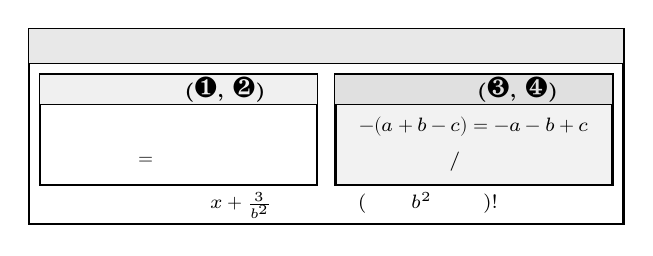
\begin{tikzpicture}[x=1cm, y=1cm, every node/.style={font=\scriptsize, text=black}]
  \draw[black, line width=0.9pt] (0,0) rectangle (7.55,2.48);
  \fill[gray!18] (0,2.04) rectangle (7.55,2.48);
  \draw[black, line width=0.6pt] (0,2.04) -- (7.55,2.04);
  \node at (3.775,2.26) {\textbf{សង្ខេបពហុធា ដឺក្រេនៃពហុធា និងក្បួនបូកដកពហុធា}};

  % Left: Polynomial & Degree
  \draw[black, line width=0.8pt] (0.14,0.50) rectangle (3.66,1.90);
  \fill[gray!12] (0.14,1.52) rectangle (3.66,1.90);
  \draw[black, line width=0.55pt] (0.14,1.52) -- (3.66,1.52);
  \node at (1.90,1.71) {\textbf{ពហុធា និងដឺក្រេ (\cnum{1}, \cnum{2})}};
  \node at (1.90,1.24) {ផលបូកឯកធាមិនដូចគ្នា};
  \node at (1.90,0.80) {ដឺក្រេ $=$ ដឺក្រេតួខ្ពស់ជាងគេ};

  % Right: Add & Subtract Polynomials
  \draw[black, line width=0.95pt, fill=gray!10] (3.89,0.50) rectangle (7.41,1.90);
  \fill[gray!24] (3.89,1.52) rectangle (7.41,1.90);
  \draw[black, line width=0.6pt] (3.89,1.52) -- (7.41,1.52);
  \node at (5.65,1.71) {\textbf{បូក និងដកពហុធា (\cnum{3}, \cnum{4})}};
  \node at (5.65,1.24) {$-(a+b-c) = -a-b+c$};
  \node at (5.65,0.80) {ផ្គុំបូក/ដកតែឯកធាដូចគ្នា};

  \node at (3.775,0.24) {\textbf{ប្រយ័ត្ន៖} $x + \tfrac{3}{b^2}$ មិនមែនពហុធាទេ (មានអថេរ $b^2$ នៅភាគបែង)!};
\end{tikzpicture}}

% ៤. E4 Elaborate: តារាងរៀបលំដាប់កើន/ចុះ និងគណនា M+N, M-N (ទំ.៥៨--៥៩)
\newcommand{\figElaborateALGFiveThree}{%
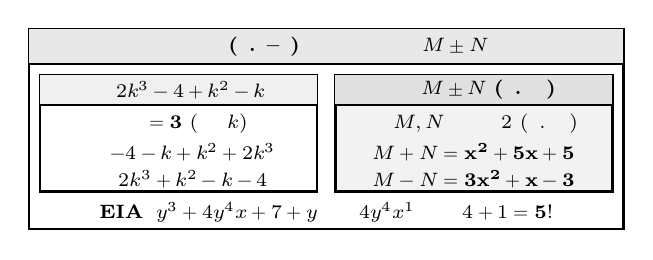
\begin{tikzpicture}[x=1cm, y=1cm, every node/.style={font=\scriptsize, text=black}]
  \draw[black, line width=0.9pt] (0,0) rectangle (7.55,2.54);
  \fill[gray!18] (0,2.10) rectangle (7.55,2.54);
  \draw[black, line width=0.6pt] (0,2.10) -- (7.55,2.10);
  \node at (3.775,2.32) {\textbf{លំហាត់គំរូ (ទំ.៥៨--៥៩)៖ រៀបលំដាប់ពហុធា និង $M \pm N$}};

  % Left: Ordering 2k^3 - 4 + k^2 - k
  \draw[black, line width=0.8pt] (0.14,0.48) rectangle (3.66,1.96);
  \fill[gray!12] (0.14,1.58) rectangle (3.66,1.96);
  \draw[black, line width=0.55pt] (0.14,1.58) -- (3.66,1.58);
  \node at (1.90,1.77) {\textbf{រៀប $2k^3 - 4 + k^2 - k$}};
  \node at (1.90,1.34) {ដឺក្រេ $= \mathbf{3}$ (អថេរ $k$)};
  \node at (1.90,0.98) {កើន៖ $-4 - k + k^2 + 2k^3$};
  \node at (1.90,0.64) {ចុះ៖ $2k^3 + k^2 - k - 4$};

  % Right: M+N and M-N
  \draw[black, line width=0.95pt, fill=gray!10] (3.89,0.48) rectangle (7.41,1.96);
  \fill[gray!24] (3.89,1.58) rectangle (7.41,1.96);
  \draw[black, line width=0.6pt] (3.89,1.58) -- (7.41,1.58);
  \node at (5.65,1.77) {\textbf{គណនា $M \pm N$ (ទំ.៥៩ ក)}};
  \node at (5.65,1.34) {ឱ្យ $M, N$ ដឺក្រេទី $2$ (ទំ.៥៩ ក)};
  \node at (5.65,0.98) {$M+N = \mathbf{x^2 + 5x + 5}$};
  \node at (5.65,0.64) {$M-N = \mathbf{3x^2 + x - 3}$};

  \node at (3.775,0.22) {\textbf{\en{EIA}៖} $y^3 + 4y^4x + 7 + y$ មានតួ $4y^4x^1$ ដឺក្រេ $4+1 = \mathbf{5}$!};
\end{tikzpicture}}

% ៥. E5 Evaluate: ជម្រើសវិនិច្ឆ័យ A-D គណនា (4x^2 - 3x + 1) - (x^2 - 5x + 4)
\newcommand{\figExitALGFiveThree}{%
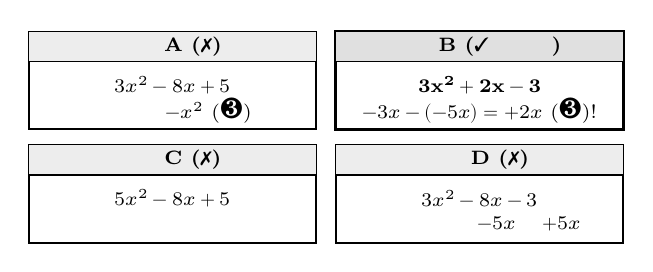
\begin{tikzpicture}[x=1cm, y=1cm, every node/.style={font=\scriptsize, text=black}]
  % Choice A
  \draw[black, line width=0.8pt] (0,1.44) rectangle (3.65,2.68);
  \fill[gray!14] (0,2.30) rectangle (3.65,2.68);
  \draw[black, line width=0.5pt] (0,2.30) -- (3.65,2.30);
  \node at (1.825,2.49) {\textbf{ជម្រើស \en{A} (\ding{55})}};
  \node at (1.825,2.00) {$3x^2 - 8x + 5$};
  \node at (1.825,1.68) {ប្ដូរតែតួទី១ $-x^2$ (\cnum{3})};

  % Choice B (Correct)
  \draw[black, line width=1.05pt] (3.90,1.44) rectangle (7.55,2.68);
  \fill[gray!24] (3.90,2.30) rectangle (7.55,2.68);
  \draw[black, line width=0.6pt] (3.90,2.30) -- (7.55,2.30);
  \node at (5.725,2.49) {\textbf{ជម្រើស \en{B} (\ding{51} ត្រឹមត្រូវ)}};
  \node at (5.725,2.00) {$\mathbf{3x^2 + 2x - 3}$};
  \node at (5.725,1.68) {$-3x - (-5x) = +2x$ (\cnum{3})!};

  % Choice C
  \draw[black, line width=0.8pt] (0,0) rectangle (3.65,1.24);
  \fill[gray!14] (0,0.86) rectangle (3.65,1.24);
  \draw[black, line width=0.5pt] (0,0.86) -- (3.65,0.86);
  \node at (1.825,1.05) {\textbf{ជម្រើស \en{C} (\ding{55})}};
  \node at (1.825,0.56) {$5x^2 - 8x + 5$};
  \node at (1.825,0.24) {ច្រឡំបូកពហុធាទាំងពីរ};

  % Choice D
  \draw[black, line width=0.8pt] (3.90,0) rectangle (7.55,1.24);
  \fill[gray!14] (3.90,0.86) rectangle (7.55,1.24);
  \draw[black, line width=0.5pt] (3.90,0.86) -- (7.55,0.86);
  \node at (5.725,1.05) {\textbf{ជម្រើស \en{D} (\ding{55})}};
  \node at (5.725,0.56) {$3x^2 - 8x - 3$};
  \node at (5.725,0.24) {ភ្លេចប្ដូរសញ្ញាតួ $-5x$ ទៅ $+5x$};
\end{tikzpicture}}

\begin{document}
\fontsize{10pt}{15.2pt}\selectfont

% ============================================================================
% ក្បាលរដ្ឋបាល (Administrative Header — តាមគំរូ ls_plan.tex)
% ============================================================================
{\centering
  {\muol\fontsize{11pt}{16pt}\selectfont ព្រះរាជាណាចក្រកម្ពុជា\par}
  {\muol\fontsize{11pt}{16pt}\selectfont ជាតិ សាសនា ព្រះមហាក្សត្រ\par}
  \vspace{-3pt}{\khmflourish\par}
}

\vspace{1pt}
{\muol\fontsize{10pt}{15.5pt}\selectfont
មន្ទីរអប់រំ យុវជន និងកីឡា ខេត្តកំពង់ធំ\par
ការិយាល័យអប់រំ យុវជន និងកីឡា ស្រុកកំពង់ស្វាយ\par
អនុវិទ្យាល័យព្រះក្រសាំង\par}

\vspace{2pt}
{\centering{\muol\fontsize{11.5pt}{17pt}\selectfont កិច្ចតែងការបង្រៀន\par}}
\vspace{2pt}

% --- ព័ត៌មានទូទៅ ---
{\hspace*{2.8cm}\renewcommand{\arraystretch}{1.08}
\begin{tabular}{@{}l@{\hspace{0.35cm}}p{2.9cm}@{\hspace{0.15cm}}c@{\hspace{0.25cm}}l@{}}
  - & មុខវិជ្ជា & : & គណិតវិទ្យា ថ្នាក់ទី៨ (ពីជគណិត) \\
  - & ចំណងជើងមេរៀន & : & មេរៀនទី៥៖ កន្សោមពីជគណិត \\
  - & ចំណងជើងរង & : & ២.១ សញ្ញាណពហុធា, ២.២ ដឺក្រេនៃពហុធា និង ២.៣ វិធីបូកនិងដកពហុធា \\
  - & រយៈពេល & : & ១ ម៉ោងសិក្សា (៥០ នាទី) \\
  - & បង្រៀនដោយ & : & ហុក ប៊ុនថែន \\
  - & កាលបរិច្ឆេទ & : & ថ្ងៃចន្ទ ទី៧ ខែធ្នូ ឆ្នាំ២០២៦ \\
\end{tabular}\par}

\vspace{2pt}

% --- I. វត្ថុបំណង ---
{\muol\fontsize{10pt}{15.5pt}\selectfont \enbf{I.} វត្ថុបំណង\par}
\vspace{1pt}
{\renewcommand{\arraystretch}{1.10}
\begin{tabular}{@{}p{0.55cm}@{}p{2.35cm}@{\hspace{0.15cm}}c@{\hspace{0.25cm}}p{14.95cm}@{}}
  \hfill\wcirc\hspace{0.2cm} & វិជ្ជាសម្បទា & : & សិស្សប្រាប់និយមន័យពហុធា (ទ្វេធានិងត្រីធា) ដឺក្រេនៃពហុធា ការរៀបតាមលំដាប់កើន/ចុះ និងក្បួនបូកនិងដកពហុធាបានត្រឹមត្រូវ (ទំ.៥៦--៥៩) ។ \\
  \hfill\wcirc\hspace{0.2cm} & បំណិនសម្បទា & : & សិស្សកំណត់អថេរ ចំនួនតួ ដឺក្រេ រៀបលំដាប់ពហុធា និងគណនាផលបូកនិងផលដកពហុធាតាមជួរដេកនិងជួរឈរលើសន្លឹកកិច្ចការបានត្រឹមត្រូវ ។ \\
  \hfill\wcirc\hspace{0.2cm} & ចរិយាសម្បទា & : & សិស្សមានទម្លាប់ប្រុងប្រយ័ត្នខ្ពស់ចំពោះការប្ដូរសញ្ញាគ្រប់តួក្នុងវង់ក្រចកក្រោយសញ្ញាដក និងរៀបខ្ទង់ដឺក្រេឱ្យមានរបៀបរៀបរយ ។ \\
\end{tabular}\par}

\vspace{2pt}

% --- II. សម្ភារៈឧបទេស ---
{\muol\fontsize{10pt}{15.5pt}\selectfont \enbf{II.} សម្ភារៈឧបទេស\par}
\vspace{1pt}
\hspace*{0.55cm}$\bullet$\ សៀវភៅសិក្សាគោលថ្នាក់ទី៨ (ទំ.៥៦--៥៩, ៧២--៧៣) ក្ដារខៀន ដីស/ហ្វឺត បន្ទាត់ត្រង់ និង\textbf{សន្លឹកកិច្ចការសិស្សបំពេញចន្លោះ ស-ខ្មៅ} (កូដ \en{ALG53} ទំព័រ ១--២ សម្រាប់សិស្ស និងទំព័រ ៣ ប្លង់ក្ដារខៀន/ចម្លើយគ្រូ — គ្មានប្រើ \en{LCD})\par

\vspace{2pt}

% --- III. វិធីសាស្រ្តបង្រៀន ---
{\muol\fontsize{10pt}{15.5pt}\selectfont \enbf{III.} វិធីសាស្រ្តបង្រៀន\par}
\vspace{1pt}
{\renewcommand{\arraystretch}{1.08}
\begin{tabular}{@{}p{0.55cm}@{}p{2.35cm}@{\hspace{0.15cm}}c@{\hspace{0.25cm}}p{14.95cm}@{}}
  \hfill$\bullet$\hspace{0.2cm} & គោលវិធី & : & សិស្សមជ្ឈមណ្ឌល (សន្លឹកកិច្ចការបំពេញចន្លោះជាគោល + ការពិភាក្សាជាក្រុមតូច ៣ នាក់) \\
  \hfill$\bullet$\hspace{0.2cm} & យុទ្ធវិធីបង្រៀន & : & គំរូស្ថាបនានិយម \en{5Es} រួមបញ្ចូល \textbf{អន្ទាក់សញ្ញាដកមុខវង់ក្រចក} និង \textbf{ការតម្រង់ខ្ទង់ឯកធាដូចគ្នាតាមជួរឈរ (ថែមតួ $0x$)} \\
\end{tabular}\par}

\vspace{2pt}

% --- IV. ដំណើរការបង្រៀន ---
{\muol\fontsize{10pt}{15.5pt}\selectfont \enbf{IV.} ដំណើរការបង្រៀន\par}

{\renewcommand{\arraystretch}{1.15}
\begin{longtable}{|L{5.50cm}|L{7.90cm}|L{4.80cm}|}
\hline
\multicolumn{1}{|c|}{\cellcolor{headgray}\muol សកម្មភាពគ្រូ} &
\multicolumn{1}{c|}{\cellcolor{headgray}\muol ខ្លឹមសារមេរៀន} &
\multicolumn{1}{c|}{\cellcolor{headgray}\muol សកម្មភាពសិស្ស} \\
\hline
\endfirsthead

\hline
\multicolumn{1}{|c|}{\cellcolor{headgray}\muol សកម្មភាពគ្រូ} &
\multicolumn{1}{c|}{\cellcolor{headgray}\muol ខ្លឹមសារមេរៀន} &
\multicolumn{1}{c|}{\cellcolor{headgray}\muol សកម្មភាពសិស្ស} \\
\hline
\endhead

% ==================== ជំហានទី១ (2min) ====================
\stepheader{ជំហានទី១ \enbf{(}រដ្ឋបាលថ្នាក់\enbf{)}}
$\bullet$ ពិនិត្យវត្តមាន អនាម័យ និងសណ្ដាប់ធ្នាប់ថ្នាក់រៀន \par
$\bullet$ រៀបចំក្រុមតូច ៣ នាក់ និងចែក\textbf{សន្លឹកកិច្ចការសិស្ស (\en{ALG53} ទំព័រ ១–២)}
&
$\bullet$ រដ្ឋបាលថ្នាក់ អនាម័យ និងវិន័យសិក្សា \par
$\bullet$ ចែកសន្លឹកកិច្ចការម្នាក់ ១ សន្លឹក សម្រាប់បំពេញតាមដំណាក់កាល \en{E1--E5}
&
$\circ$ ប្រធានថ្នាក់រាយការណ៍វត្តមានសិស្ស \par
$\circ$ ទទួលសន្លឹកកិច្ចការ សរសេរឈ្មោះ និងអង្គុយតាមក្រុម ៣ នាក់ \\
\hline

% ==================== ជំហានទី២ (9min: កំណែ <=3m + រំលឹក 3m + E1 3m) ====================
\stepheader{ជំហានទី២ \enbf{(}កិច្ចការផ្ទះ \enbf{+} ទំនាក់ទំនងមេរៀនថ្មី\enbf{)}}
\ditem \textbf{កំណែកិច្ចការផ្ទះ ($\le\text{\enbf{3\,min}}$)} \par
$\bullet$ ហៅសិស្ស ២ នាក់ឡើងកែលំហាត់ទំ.៥៤–៥៦ និងទំ.៧២ \#3 ក លើក្ដារខៀន
&
{\centering\redsub{កំណែកិច្ចការផ្ទះ (ទំ.៥៤–៥៦ និង ទំ.៧២ \#3 ក)}\par}
$\bullet$ \textbf{បូកដក៖} ទំ.៥៤ (ច) $= \mathbf{7ac^2b^3}$; \quad ទំ.៧២ \#3 ក) $3x^2+7x^2-5x^2 = \mathbf{5x^2}$ \par
$\bullet$ \textbf{គុណចែក៖} ទំ.៥៥ (គ) $= \mathbf{\tfrac{3}{2}a^3b^5}$; \ ទំ.៥៦ (ង) $= \mathbf{x^2b^2}$; \ (ច) $= \mathbf{27b^2}$
&
$\circ$ ផ្ទៀងចម្លើយ និងកែតម្រូវចូលសៀវភៅកិច្ចការផ្ទះ \\[3pt]

\ditem \textbf{រំលឹកមេរៀនទាក់ទង (\enbf{3min})} \par
$\bullet$ សួរ៖ «តើ $-8x^2$ និង $3xy$ អាចបូកបង្រួមជាឯកធាតែមួយបានឬទេ? ចុះ $-(a+b-c)$ ពេលលុបវង់ក្រចកស្មើអ្វី?»
&
{\centering\redsub{រំលឹកឯកធាមិនដូចគ្នា និងការលុបវង់ក្រចក}\par}
$\bullet$ $-8x^2$ និង $3xy$ ជា\textbf{ឯកធាមិនដូចគ្នា} មិនអាចបង្រួមចូលគ្នាបានទេ \par
$\bullet$ លុបវង់ក្រចកក្រោយសញ្ញាដក៖ $-(a + b - c) = -a - b + c$
&
$\circ$ ឆ្លើយ៖ «បង្រួមមិនបានទេ; ត្រូវប្ដូរសញ្ញាគ្រប់តួក្នុងវង់ក្រចក!» \\[3pt]

\fiveE{E1 - Engage (3min)} \timenote{(កុំទាន់ផ្ដល់ចម្លើយ)} \par
\ditem \textbf{បេសកកម្មអន្ទាក់សញ្ញាដកមុខវង់ក្រចក (សន្លឹកកិច្ចការ \en{E1})} \par
$\bullet$ ឱ្យសិស្សអានប្រអប់ \en{E1} ហើយគូសជ្រើសរើសរវាង\textbf{សិស្ស ក} និង\textbf{សិស្ស ខ}
&
\redsub{បេសកកម្ម \en{E1}៖ គណនា $(3x^2 - 2x + 7) - (x^2 + 4x + 5)$} \par
$\bullet$ \textbf{សិស្ស ក} ប្ដូរតែតួទី១ បាន $3x^2-2x+7-x^2+4x+5 = 2x^2+2x+12$! \par
$\bullet$ \textbf{សិស្ស ខ} ប្ដូរគ្រប់តួក្នុងវង់ក្រចក បាន $2x^2 - 6x + 2$! តើអ្នកណាត្រូវ?
&
$\circ$ ពិភាក្សាជាគូ និងគូស \ding{51} ក្នុងប្រអប់ \en{E1} លើសន្លឹកកិច្ចការ \\[3pt]

&
\cfig{\figEngageALGFiveThree}
& \\
\hline

% ==================== ជំហានទី៣ (17min: E2 11m + E3 6m) ====================
\stepheader{ជំហានទី៣ \enbf{(}ខ្លឹមសារមេរៀនថ្មី\enbf{)}}
\fiveE{E2 - Explore (11min)} \par
$\bullet$ សរសេរចំណងជើងរង \textbf{២. ពហុធា (២.១–២.៣)} លើក្ដារខៀន \par
\ditem \textbf{សកម្មភាព ១៖ សញ្ញាណពហុធា និងដឺក្រេនៃពហុធា (ទំ.៥៦–៥៨, \enbf{5min}, \en{E2-A})} \par
$\bullet$ ឱ្យសិស្សបំពេញបរិមាត្រត្រីកោណ ចំនួនតួ និងដឺក្រេនៃពហុធាលើ \en{E2-A}
&
២. ពហុធា \quad (២.១ សញ្ញាណពហុធា, ២.២ ដឺក្រេនៃពហុធា) \par
$\bullet$ \textbf{សញ្ញាណពហុធា (ទំ.៥៦–៥៧)៖} បរិមាត្រត្រីកោណ $3y + 2x + 8$ ជាផលបូកឯកធាមិនដូចគ្នា ហៅថា \textbf{ពហុធា} (២ តួ ហៅ \textbf{ទ្វេធា} ដូចជា $3x-8$; ៣ តួ ហៅ \textbf{ត្រីធា} ដូចជា $5x^2-2x+7$; ឯ $x+\tfrac{3}{b^2}$ មិនមែនពហុធាទេ) \par
$\bullet$ \textbf{ដឺក្រេ និងលំដាប់ (ទំ.៥៧–៥៨)៖} $-x^2-2x^2y-1$ មានដឺក្រេខ្ពស់ស្មើ $\mathbf{3}$; \ $11+5x^2-3x$ មានដឺក្រេ $\mathbf{2}$ (កើន៖ $11-3x+5x^2$, ចុះ៖ $5x^2-3x+11$)
&
$\circ$ បំពេញបរិមាត្រ ចំនួនតួ និងរៀបលំដាប់កើន/ចុះលើ \en{E2-A} \\[3pt]

\ditem \textbf{សកម្មភាព ២៖ វិធីបូក និងដកពហុធា (ទំ.៥៨–៥៩, \enbf{6min}, \en{E2-B})} \par
$\bullet$ ឱ្យសិស្សគណនា $A+B, E-F$ តាមជួរដេក និងគំរូជួរឈរលើ \en{E2-B}
&
២.៣ វិធីបូកនិងដកពហុធា (ទំ.៥៨–៥៩) \par
$\bullet$ \textbf{ជួរដេក៖} $A+B = (2a^2+3a-4)+(5a^2-7a+6) = \mathbf{7a^2-4a+2}$; \quad $E-F = (3x^2-2x+7)-(x^2+4x+5) = \mathbf{2x^2-6x+2}$ \par
$\bullet$ \textbf{ជួរឈរ (ទំ.៥៨–៥៩)៖} $A = 5x^3-2x^2+7x+4, \ B = 2x^3+4x^2-6 \implies A+B = \mathbf{7x^3+2x^2+7x-2}$ និង $A-B = \mathbf{3x^3-6x^2+7x+10}$
&
$\circ$ គណនាផលបូកនិងផលដកពហុធាទាំងជួរដេក និងជួរឈរ \\[3pt]

&
\cfig{\figPolyExploreALGFiveThree}
& \\[3pt]

% --- E3 Explain (6min) ---
\fiveE{E3 - Explain (6min)} \par
$\bullet$ ដឹកនាំសិស្សសង្ខេបនិយមន័យពហុធា ដឺក្រេ និងក្បួនបូកដកពហុធា (ទំ.៥៧–៥៨)
&
$\bullet$ \textbf{និយមន័យ និងក្បួនគោល (ទំ.៥៧–៥៨)៖} \par
\hspace*{0.15cm}១) \textbf{ពហុធា៖} ផលបូកនៃពីរ ឬច្រើនឯកធាមិនដូចគ្នា (២ តួ $=$ ទ្វេធា, ៣ តួ $=$ ត្រីធា) \par
\hspace*{0.15cm}២) \textbf{ដឺក្រេនៃពហុធា៖} គឺជា\graybox{ដឺក្រេរបស់តួដែលមានដឺក្រេខ្ពស់ជាងគេ} \par
\hspace*{0.15cm}៣) \textbf{បូក/ដកពីរពហុធា៖} លុបវង់ក្រចកឱ្យត្រូវសញ្ញា រួច\graybox{បូកឬដកឯកធាដូចគ្នា}
&
$\circ$ បំពេញប្រអប់និយមន័យទាំង ៣ លើសន្លឹកកិច្ចការ \en{E3} \\[3pt]

$\bullet$ ភ្ជាប់\textbf{ធនាគារហេតុផល \cnum{1}--\cnum{4}} លើក្ដារខៀន និងសន្លឹកកិច្ចការ
&
\textbf{ធនាគារហេតុផល (\en{Warrant Bank})៖} \par
\cnum{1} \textbf{លក្ខខណ្ឌពហុធា៖} គ្រប់តួទាំងអស់ត្រូវតែជាឯកធា (គ្មានអថេរនៅភាគបែង) \par
\cnum{2} \textbf{ដឺក្រេពហុធា៖} យកដឺក្រេអតិបរមានៃតួ ($\max$) ហាមបូកដឺក្រេគ្រប់តួបញ្ចូលគ្នា
&
$\circ$ ផ្ទៀងលេខកូដ \cnum{1}--\cnum{2} លើសន្លឹកកិច្ចការ \\[3pt]

&
\cnum{3} \textbf{ដកពហុធា៖} សញ្ញាដកមុខវង់ក្រចក ប្ដូរសញ្ញា\textbf{គ្រប់តួទាំងអស់}ក្នុងវង់ក្រចក \par
\cnum{4} \textbf{តម្រង់ខ្ទង់ជួរឈរ៖} រៀបតាមដឺក្រេចុះ និងទុកចន្លោះ $0x^k$ ចំពោះខ្ទង់ដែលបាត់
&
$\circ$ ផ្ទៀងលេខកូដ \cnum{3}--\cnum{4} លើសន្លឹកកិច្ចការ \\[3pt]

&
\cfig{\figRulePolyALGFiveThree}
& \\
\hline

% ==================== ជំហានទី៤ (20min: E4 10m + E5 10m) ====================
\stepheader{ជំហានទី៤ \enbf{(}ពង្រីកចំណេះដឹង\enbf{)}}
\fiveE{E4 - Elaborate (10min)} \par
\ditem \textbf{លំហាត់គំរូ៖ រៀបលំដាប់ពហុធា និងគណនា $M\pm N$ (ទំ.៥៧–៥៩)} \par
$\bullet$ ឱ្យសិស្សបំពេញតារាងរៀបលំដាប់ និងគណនា $M+N, M-N$ លើ \en{E4}
&
{\muol លំហាត់គំរូ} \textbf{(ទំ.៥៧–៥៩)៖} \par
$\bullet$ \textbf{១) តារាងដឺក្រេ និងលំដាប់ (ទំ.៥៨)៖} \par
\hspace*{0.2cm}-- $2k^3 - 4 + k^2 - k$៖ ដឺក្រេ $\mathbf{3}$, កើន $-4-k+k^2+2k^3$, ចុះ $2k^3+k^2-k-4$ \par
\hspace*{0.2cm}-- $y^3 + 4y^4x + 7 + y$៖ អថេរ $x, y$, ដឺក្រេ $\mathbf{5}$, ចុះ $4y^4x + y^3 + y + 7$ \par
$\bullet$ \textbf{២) ប្រតិបត្តិទំ.៥៩ (ក)៖} $M = 2x^2+3x+1, \ N = -x^2+2x+4$ \par
\hspace*{0.2cm}$\implies M+N = \graybox{$x^2 + 5x + 5$}$ \quad និង \quad $M-N = \graybox{$3x^2 + x - 3$}$
&
$\circ$ រៀបលំដាប់ពហុធា និងគណនាឃើញ $M+N, M-N$ \\[3pt]

&
\cfig{\figElaborateALGFiveThree}
& \\[3pt]

$\bullet$ សួរសំណួរឆ្លុះបញ្ចាំង \textbf{\en{EIA Looking-Back} (1min)}
&
\textbf{\en{EIA Looking-Back}៖} «ហេតុអ្វីពហុធា $y^3 + 4y^4x + 7 + y$ មានដឺក្រេស្មើ $5$ មិនមែនស្មើ $4$ ទេ?» ($\to$ ព្រោះតួ $4y^4x = 4y^4x^1$ មានផលបូកនិទស្សន្ត $4 + 1 = 5$ ខ្ពស់ជាងគេ!)
&
$\circ$ ពន្យល់ថាត្រូវបូកនិទស្សន្តគ្រប់អថេរក្នុងតួ $4y^4x$ \\[3pt]

% --- E5 Evaluate (10min) ---
\fiveE{E5 - Evaluate (10min)} \par
\ditem \textbf{ប្រតិបត្តិជាក្រុមតូច ៣ នាក់ (4min, សន្លឹកកិច្ចការ \en{E5})} \par
$\bullet$ ឱ្យសិស្សដោះស្រាយប្រតិបត្តិទំ.៥៧ (ក) ទំ.៥៨ (គ) និងទំ.៥៩ (ខ)
&
{\muol លំហាត់ប្រតិបត្តិ} \textbf{(ទំ.៥៧–៥៩)៖} \par
$\bullet$ \textbf{១) ទំ.៥៧ (ក) និង ទំ.៥៨ (គ)៖} $6x^3+2xy-4$ (អថេរ $x,y$, $3$ តួ); \ $a^2+2ab+c^2d$ (ដឺក្រេ $\mathbf{3}$) \par
$\bullet$ \textbf{២) ទំ.៥៩ (ខ)៖} $M = 12a^2+2ab+54, \ N = 9a^2-4ab-25$ \par
\hspace*{0.2cm}$\implies M+N = \mathbf{21a^2 - 2ab + 29}$; \quad $M-N = \mathbf{3a^2 + 6ab + 79}$
&
$\circ$ គណនាជាក្រុមឃើញដឺក្រេ $3$ និង $M\pm N$ ត្រឹមត្រូវ \\[3pt]

$\bullet$ ឱ្យក្រុមសិស្សផ្ទៀងផ្ទាត់និង\textbf{បិទបេសកកម្ម \en{E1} (2min)}
&
$\bullet$ \textbf{បិទបេសកកម្ម \en{E1}៖} សិស្ស ខ ត្រឹមត្រូវ! $E - F = (3x^2-x^2)+(-2x-4x)+(7-5) = \mathbf{2x^2 - 6x + 2}$!
&
$\circ$ បិទបេសកកម្ម \en{E1} ឃើញសិស្ស ខ ត្រឹមត្រូវ \\[3pt]

\ditem \textbf{សំណួរវិនិច្ឆ័យ \en{A--D} និងសំបុត្រចេញ (4min)} \par
$\bullet$ ឱ្យសិស្សគូសរង្វង់ជម្រើសត្រូវលើសន្លឹកកិច្ចការ រួចលើកម្រាមដៃ ១--៤
&
{\centering\textbf{សំណួរវិនិច្ឆ័យ \en{A--D}៖ គណនាផលដក $(4x^2 - 3x + 1) - (x^2 - 5x + 4)$}\par}
{\centering \enbf{A.}\ $3x^2-8x+5$ \quad \enbf{B.}\ $3x^2+2x-3$ \quad \enbf{C.}\ $5x^2-8x+5$ \quad \enbf{D.}\ $3x^2-8x-3$\par}
&
$\circ$ គណនា និងលើកម្រាមដៃ ២ (\textbf{ជម្រើស \en{B}៖ $3x^2+2x-3$}) \\[3pt]

&
\cfig{\figExitALGFiveThree}
& \\[3pt]

$\bullet$ បញ្ជាក់ចម្លើយត្រូវ (\textbf{ជម្រើស \en{B}}) និងឱ្យបំពេញ\textbf{សំបុត្រចេញ ៦០ វិនាទី}
&
$\bullet$ \textbf{សំបុត្រចេញ៖} ពហុធា $-3x^2y + \tfrac{1}{2}y^4 - 2$ មាន $\mathbf{3}$ តួ (ត្រីធា) និងមានដឺក្រេស្មើ $\mathbf{4}$ ។
&
$\circ$ បំពេញសំបុត្រចេញលើសន្លឹកកិច្ចការមុនបញ្ចប់ម៉ោង \\
\hline

% ==================== ជំហានទី៥ (<=2min) ====================
\stepheader{ជំហានទី៥ \enbf{(}កិច្ចការផ្ទះ \enbf{+} បណ្ដាំផ្ញើ\enbf{)}}
\timenote{ចំណាយពេលឱ្យតិចបំផុតកុំឱ្យលើស 2min} \par
$\bullet$ ណែនាំប្រអប់\textbf{កិច្ចការផ្ទះ}លើសន្លឹកកិច្ចការទំព័រ ២ (ទំ.៥៩ គ និងទំ.៧២–៧៣ \#4, \#5 ខ)
&
{\centering{\muol កិច្ចការផ្ទះ} \textbf{(សៀវភៅគោល ទំ.៥៩ និង ទំ.៧២–៧៣ \#4, \#5 ខ)}\par} \par
$\bullet$ \textbf{១) ប្រតិបត្តិទំ.៥៩ (គ)៖} គណនា $M+N$ និង $M-N$ បើ $M = \tfrac{1}{2}xy^2+2xy-3, \ N = \tfrac{3}{2}xy^2-12xy-16$ ។ \par
$\bullet$ \textbf{២) លំហាត់ \#4 (ទំ.៧២) និង \#5 ខ (ទំ.៧៣)៖} គណនា $A-B, B-A$ (រៀបដឺក្រេចុះ) និង $(5a^3b^2-3ab)+(2a^3b^2-ab)$ ។
&
$\circ$ គូសចំណាំកិច្ចការផ្ទះលើសន្លឹកកិច្ចការ \\[3pt]

$\bullet$ ផ្ដាំផ្ញើឱ្យអានមុនចំណុច ២.៤–២.៥ (វិធីគុណពហុធា និងវិធីចែកពហុធា)
&
$\bullet$ \textbf{បណ្ដាំផ្ញើ៖} អានមុន \textbf{២.៤–២.៥ វិធីគុណនិងចែកពហុធា (ទំ.៥៩–៦២)} ។
&
$\circ$ កត់ត្រាបណ្ដាំផ្ញើ ទុកសន្លឹកកិច្ចការក្នុងសៀវភៅ និងជម្រាបលាគ្រូ \\
\hline
\end{longtable}}

\vspace{6pt}
% --- ហត្ថលេខា (កាលបរិច្ឆេទត្រូវគ្នា ១០០% នឹងខាងលើ) ---
{\centering
\hspace*{5.2cm}\begin{minipage}{11.5cm}
  \centering
  ថ្ងៃចន្ទ ១៣រោច ខែកត្តិក ឆ្នាំមមី អដ្ឋស័ក ពុទ្ធសករាជ ២៥៧០\par
  កំពង់ស្វាយ, ថ្ងៃទី៧ ខែធ្នូ ឆ្នាំ២០២៦\par
  \vspace{2pt}
  {\muol គ្រូបង្រៀន\par}
  \vspace{32pt}
  \hfill{\muol ហុក ប៊ុនថែន}\hspace*{1.4cm}
\end{minipage}\par}

\end{document}
